\documentclass[../relatorio.tex]{subfiles}
\begin{document}
% - estratégia utilizada
% -- arvore de parsing concreta
% -- classes
% -- hierarquia
% -- descentralização das responsabilidades
% -- diagrama de classes

No âmbito de aplicar as regras da gramática definidas anteriormente,
recorreu-se ao uso do módulo \textit{Yacc} da biblioteca \textit{PLY}. 
Deste modo, constroi-se um \textit{parser}, estabelecendo a análise 
sintática a efetuar.

\subsection{Árvore de \textit{Parsing} Concreta}

%árvore de parsing concreta

\subsection{Classes}

O diagrama de classes, na sua totalidade, encontra-se definido em \ref{sec:classes}.

% \subsubsection{Diretoria \textit{It}}

% \begin{figure}
%     \centering
%     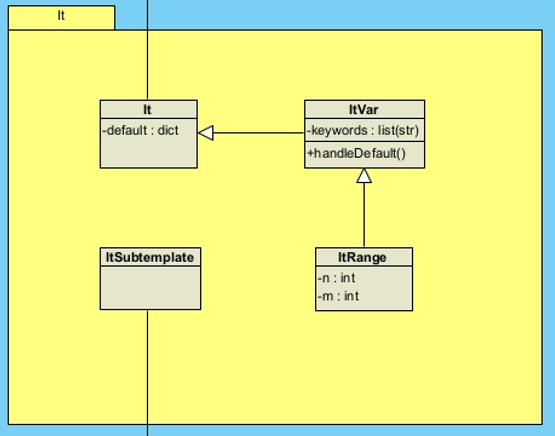
\includegraphics[width=\linewidth]{assets/dir_it.png}
%     \caption{Diretoria para a funcionalidade \textit{It}}
% \end{figure}

% \subsubsection{Diretoria \textit{Stmt}}

% \begin{figure}
%     \centering
%     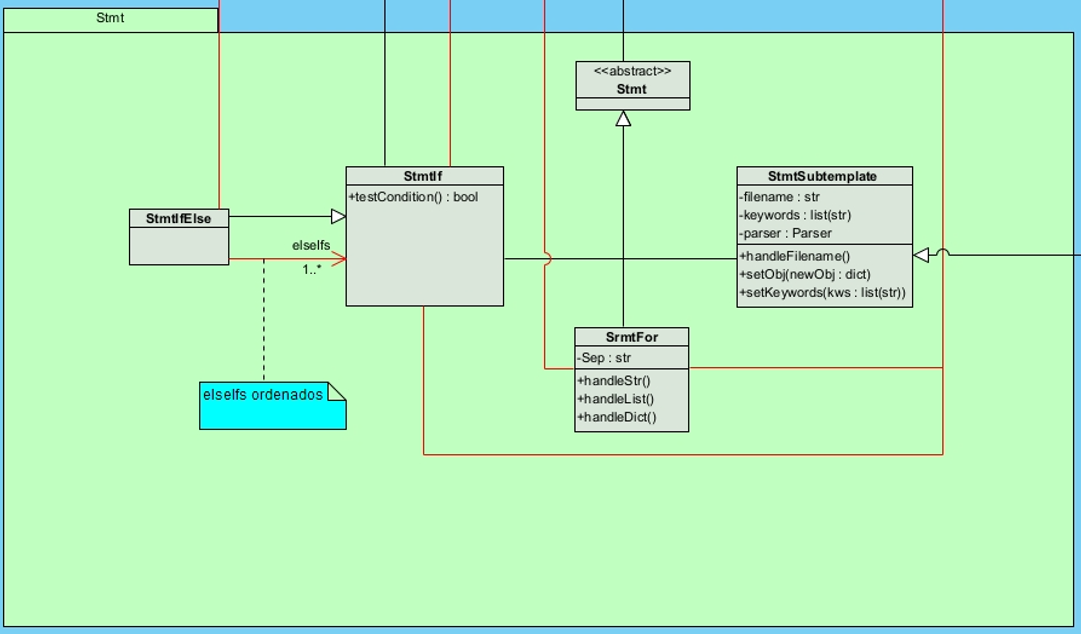
\includegraphics[width=\linewidth]{assets/dir_stmt.png}
% \end{figure}

% \subsubsection{Restantes Módulos}

% \begin{figure}
%     \centering
%     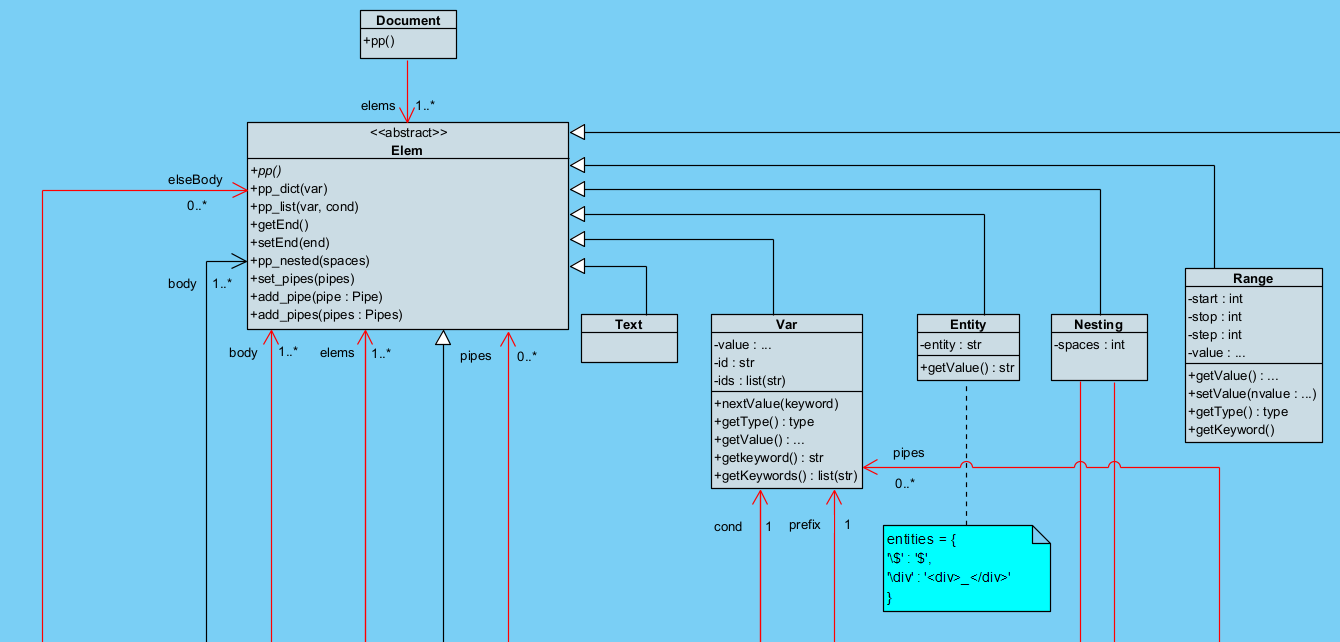
\includegraphics[width=\linewidth]{assets/dir_modules.png}
%     \caption{Classe \textit{Document} e \textit{Element}}
% \end{figure}

% \begin{figure}
%     \centering
%     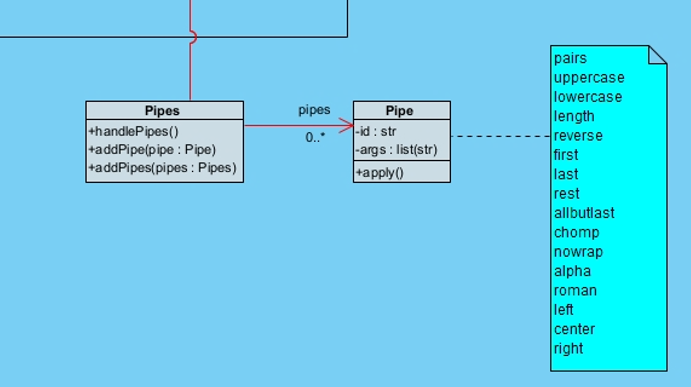
\includegraphics[width=\linewidth]{assets/pipes.png}
%     \caption{Classes independentes \textit{Pipes} e \textit{Pipe}}
% \end{figure}


\end{document}